\section{Results}

\begin{figure}[h!]
    \centering
    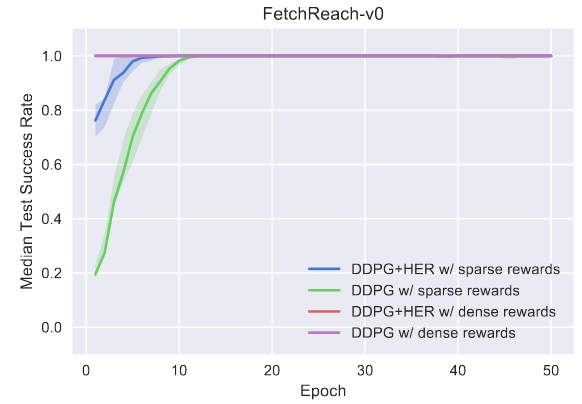
\includegraphics[width=\textwidth]{images/FRB.png}
    \caption{ToDo}
    \label{fig:HER}
\end{figure}

\begin{figure}[h!]
    \centering
    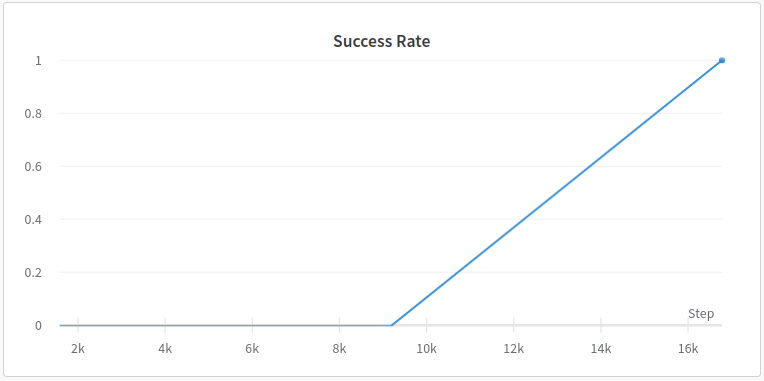
\includegraphics[width=\textwidth]{images/FRSR.png}
    \caption{ToDo}
    \label{fig:HER}
\end{figure}

\begin{figure}[h!]
    \centering
    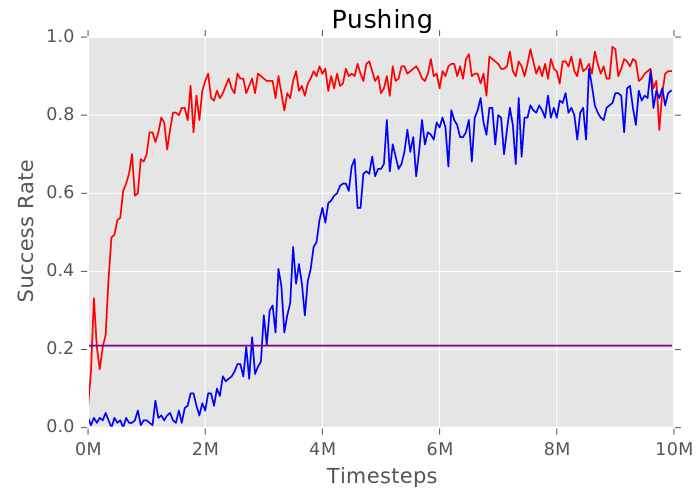
\includegraphics[width=\textwidth]{images/FPB.png}
    \caption{ToDo}
    \label{fig:HER}
\end{figure}

\begin{figure}[h!]
    \centering
    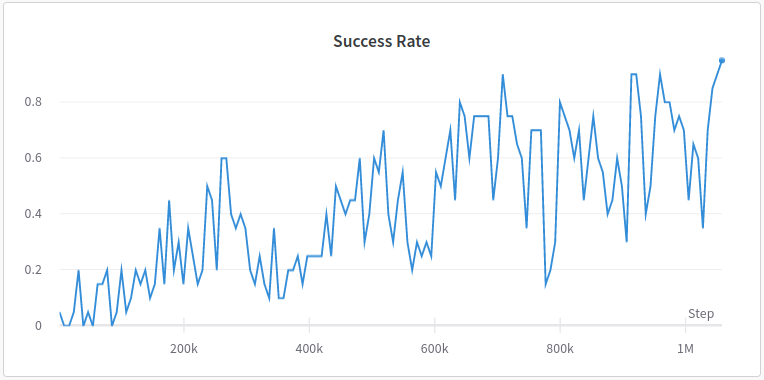
\includegraphics[width=\textwidth]{images/FPSR.png}
    \caption{ToDo}
    \label{fig:HER}
\end{figure}

\begin{figure}[h!]
    \centering
    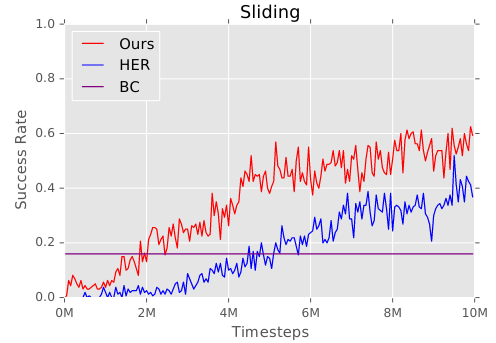
\includegraphics[width=\textwidth]{images/FSB.png}
    \caption{ToDo}
    \label{fig:HER}
\end{figure}

\begin{figure}[h!]
    \centering
    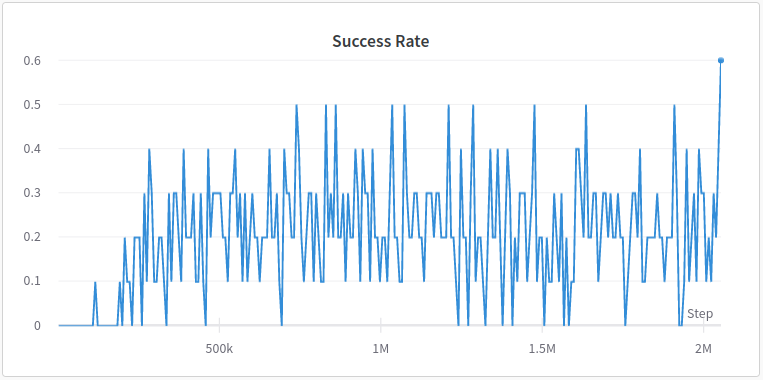
\includegraphics[width=\textwidth]{images/FSSR.png}
    \caption{ToDo}
    \label{fig:HER}
\end{figure}

\begin{figure}[h!]
    \centering
    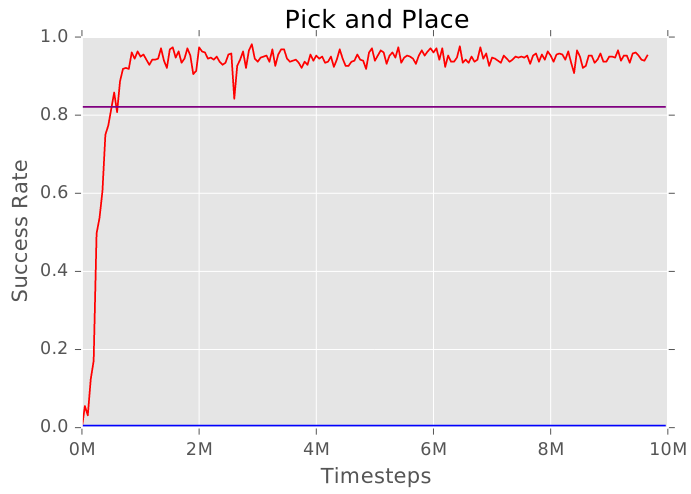
\includegraphics[width=\textwidth]{images/FPAPB.png}
    \caption{ToDo}
    \label{fig:HER}
\end{figure}

\begin{figure}[h!]
    \centering
    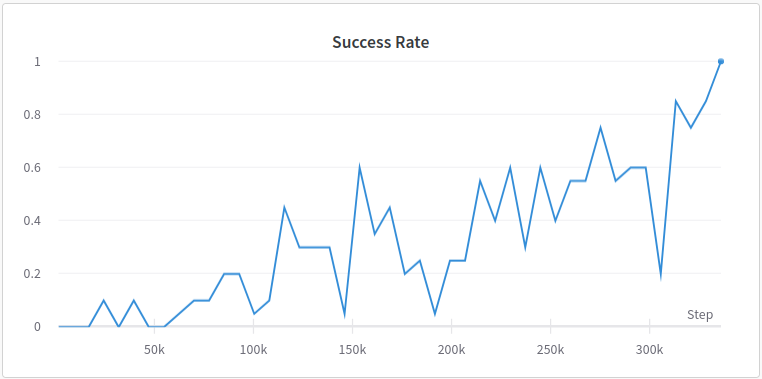
\includegraphics[width=\textwidth]{images/FPAPASR.png}
    \caption{ToDo}
    \label{fig:HER}
\end{figure}

\begin{figure}[h!]
    \centering
    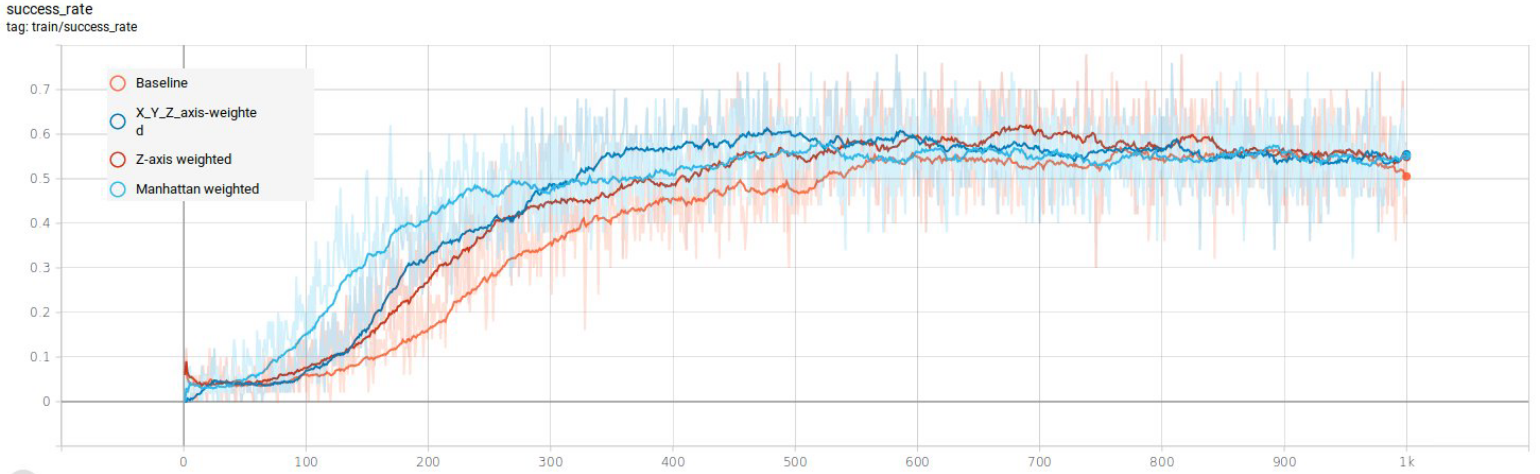
\includegraphics[width=\textwidth]{images/FPAPRRE.png}
    \caption{ToDo}
    \label{fig:HER}
\end{figure}

\begin{figure}[h!]
    \centering
    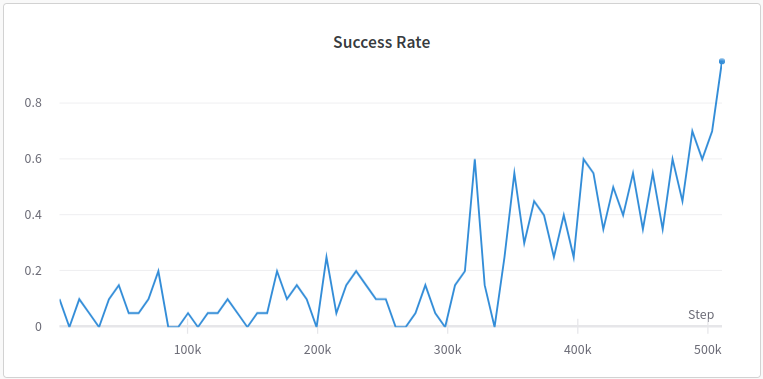
\includegraphics[width=\textwidth]{images/FPAPSSR.png}
    \caption{ToDo}
    \label{fig:HER}
\end{figure}

\begin{table}[h!]
\begin{tabular}{|c|cc|cc|c|}
\hline
Fetch Environment & Baseline I               &      & Current Implementation    &      & Speedup   \\ \hline
 & \multicolumn{1}{c|}{Timesteps} & Success Rate & \multicolumn{1}{c|}{Timesteps} & Success Rate &  \\ \hline
Reach             & \multicolumn{1}{c|}{32K} & 1.0  & \multicolumn{1}{c|}{16K}  & 1.0  & $\sim$2x  \\ \hline
Pick and Place    & \multicolumn{1}{c|}{10M} & 0.0  & \multicolumn{1}{c|}{310K} & 1.0  & -         \\ \hline
Push              & \multicolumn{1}{c|}{10M} & 0.85 & \multicolumn{1}{c|}{1.1M} & 0.95 & $\sim$10x \\ \hline
Slide             & \multicolumn{1}{c|}{10M} & 0.4  & \multicolumn{1}{c|}{2M}   & 0.6  & $\sim$5x  \\ \hline
\end{tabular}
\caption{Comparison of Current Implementation with Baseline 1}
\label{tab:my-table1}
\end{table}

\begin{table}[h!]
\begin{tabular}{|c|cc|cc|c|}
\hline
Fetch Environment & Baseline II             &     & Current Implementation    &      & Speedup  \\ \hline
               & \multicolumn{1}{c|}{Timesteps} & Success Rate & \multicolumn{1}{c|}{Timesteps} & Success Rate &          \\ \hline
Reach             & \multicolumn{1}{c|}{-}  & -   & \multicolumn{1}{c|}{16K}  & 1.0  & -        \\ \hline
Pick and Place & \multicolumn{1}{c|}{1M}        & 0.9          & \multicolumn{1}{c|}{310K}      & 1.0          & $\sim$3x \\ \hline
Push              & \multicolumn{1}{c|}{3M} & 0.9 & \multicolumn{1}{c|}{1.1M} & 0.95 & $\sim$3x \\ \hline
Slide             & \multicolumn{1}{c|}{8M} & 0.6 & \multicolumn{1}{c|}{2M}   & 0.6  & $\sim$4x \\ \hline
\end{tabular}
\caption{Comparison of Current Implementation with Baseline 2}
\label{tab:my-table2}
\end{table}

\begin{table}[h!]
\begin{tabular}{|l|l|l|}
\hline
Fetch Environment & Baseline 3   & Current Implementation \\ \hline
                  & Success Rate & Success Rate           \\ \hline
Reach             & -            & 1.0                    \\ \hline
Pick and Place    & 0.8          & 1.0                    \\ \hline
Push              & 0.2          & 0.95                   \\ \hline
Slide             & 0.2          & 0.6                    \\ \hline
\end{tabular}
\caption{}
\label{tab:my-table}
\end{table}

\begin{table}[h!]
\begin{tabular}{|c|c|c|}
\hline
Fetch Environments & Demonstrations Baseline & Demonstrations Current Implementation \\ \hline
Reach              & 100                     & 20                                    \\ \hline
Pick And Place     & 100                     & 40                                    \\ \hline
Push               & 100                     & 40                                    \\ \hline
Slide              & 100                     & 60                                    \\ \hline
\end{tabular}
\caption{Number of Demonstrations Used Compared to Baseline}
\label{tab:my-table3}
\end{table}